% Figure 2 — control-plane interposition at the tool-call boundary.
% Rebuild:
%   tectonic docs/assets/src/architecture_v2.tex
%   pdf2svg docs/assets/src/architecture_v2.pdf docs/assets/architecture_v2.svg
%
% Arxiv-style component/pipeline figure. Three horizontal bands
% (doxa / episteme / praxis). One accent colour (#7A2E2A) on the Reasoning-
% Surface Guard and the BLOCK edge. Phase 12 profile-audit loop drawn
% dashed + tan + labelled pending.

\documentclass[border=14pt,varwidth=520pt]{standalone}
\usepackage{tikz}
\usepackage{helvet}
\usepackage{amsmath}
\usepackage{amssymb}
\usepackage[T1]{fontenc}
\renewcommand{\familydefault}{\sfdefault}
\usetikzlibrary{positioning, arrows.meta, fit, backgrounds, calc}

\definecolor{ink}{HTML}{1A1A1A}
\definecolor{ink2}{HTML}{5C5C5C}
\definecolor{ink3}{HTML}{9A9A9A}
\definecolor{accent}{HTML}{7A2E2A}
\definecolor{pending}{HTML}{B5A58A}
\definecolor{bg}{HTML}{FDFDFC}

% --- font-switches (used as `{\subx text}` inside nodes) ---
\newcommand{\subx}{\color{ink2}\footnotesize}
\newcommand{\phasetagx}{\color{accent}\bfseries\footnotesize}

\begin{document}
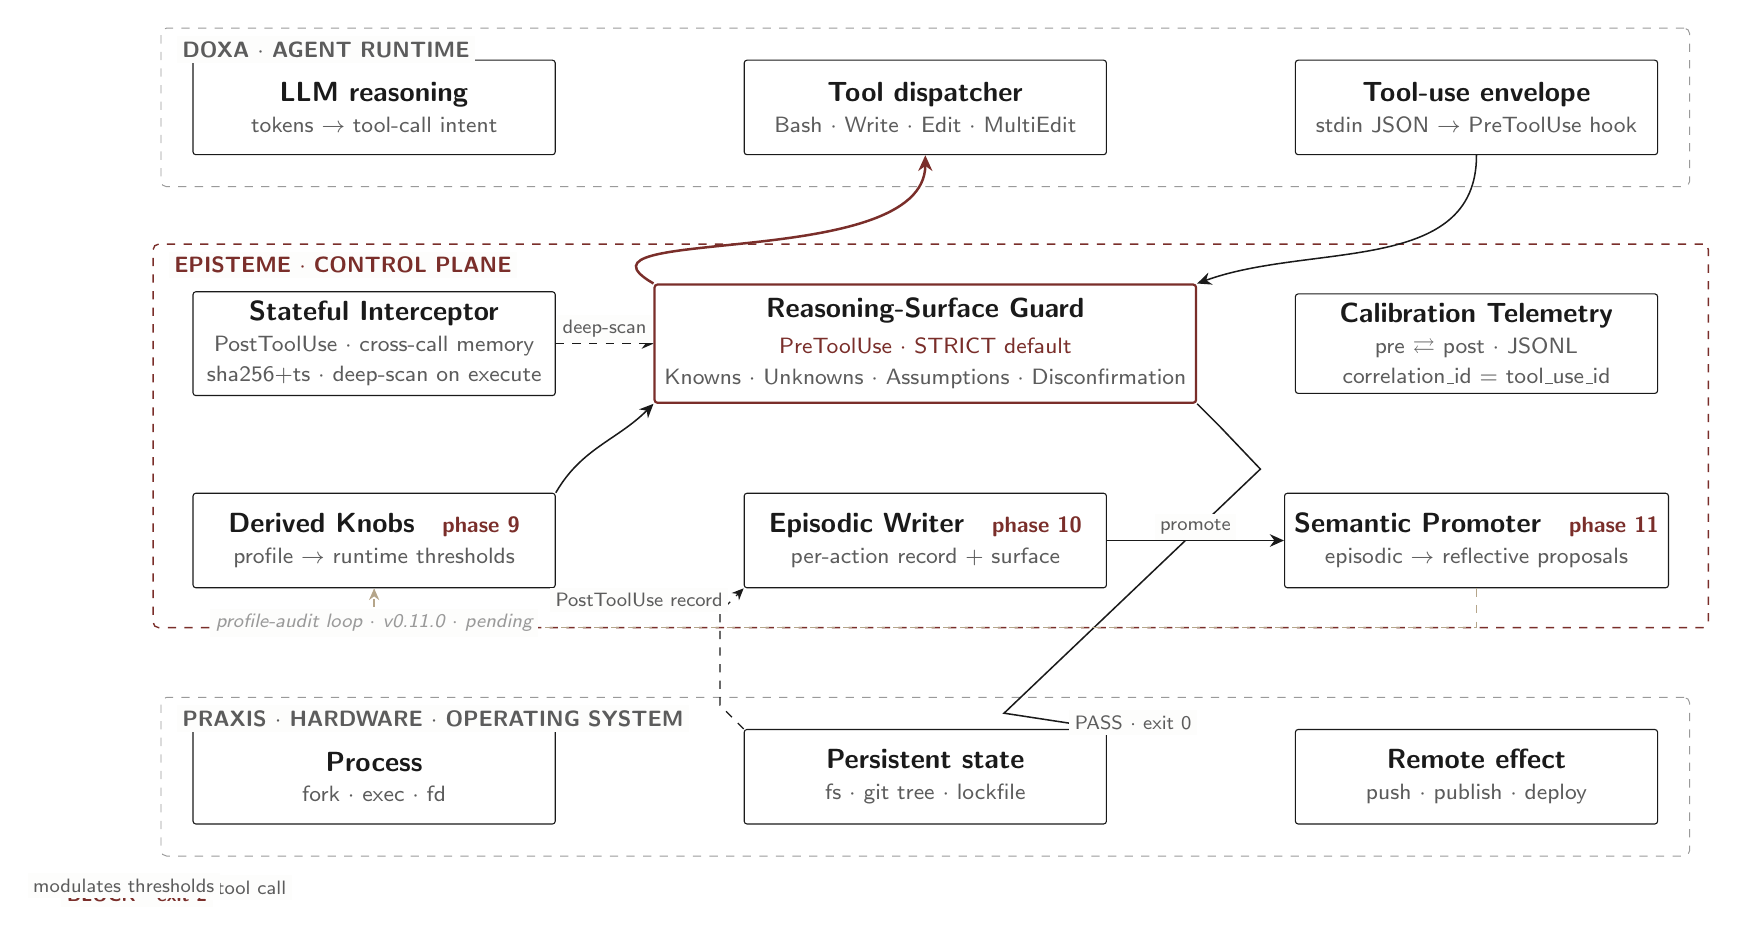
\begin{tikzpicture}[
  x=1mm, y=1mm,
  every node/.style={font=\sffamily},
  blk/.style = {
    rectangle, rounded corners=1pt,
    draw=ink, line width=0.4pt,
    fill=white,
    inner sep=3.5pt,
    text=ink,
    align=center,
    minimum width=46mm, minimum height=12mm
  },
  core/.style = {
    rectangle, rounded corners=1pt,
    draw=accent, line width=0.8pt,
    fill=white,
    inner sep=3.5pt,
    text=ink,
    align=center,
    minimum width=54mm, minimum height=15mm
  },
  band/.style = {
    rectangle, rounded corners=2pt,
    draw=ink3, line width=0.35pt, dashed,
    inner sep=4mm
  },
  band accent/.style = {
    rectangle, rounded corners=2pt,
    draw=accent, line width=0.5pt, dashed,
    inner sep=5mm
  },
  flow/.style = {-{Stealth[length=1.8mm, width=1.6mm]},
                 line width=0.55pt, color=ink},
  block/.style = {-{Stealth[length=2.0mm, width=1.8mm]},
                 line width=0.9pt, color=accent},
  feed/.style = {-{Stealth[length=1.5mm, width=1.3mm]},
                 line width=0.5pt, color=ink, dashed},
  pend/.style = {-{Stealth[length=1.5mm, width=1.3mm]},
                 line width=0.5pt, color=pending, dashed},
  lab/.style = {font=\sffamily\scriptsize, color=ink2,
                inner sep=2pt, fill=bg},
  labA/.style = {font=\sffamily\scriptsize\bfseries, color=accent,
                 inner sep=2pt, fill=bg},
  labP/.style = {font=\sffamily\scriptsize\itshape, color=ink3,
                 inner sep=2pt, fill=bg},
  sub/.style = {font=\sffamily\scriptsize, color=ink2},
  phasetag/.style = {font=\sffamily\scriptsize\bfseries, color=accent}
]

% Grid — centres in mm
%   Columns: x=20 (left) · x=90 (centre) · x=160 (right)
%   Rows:    y=100 doxa · y=70 epi row1 · y=45 epi row2 · y=15 praxis

% ─── DOXA band ─────────────────────────────────────────────────
\node[blk] (doxa_llm)  at (20,  100) {\textbf{LLM reasoning}\\[-1pt]{\subx tokens $\to$ tool-call intent}};
\node[blk] (doxa_disp) at (90,  100) {\textbf{Tool dispatcher}\\[-1pt]{\subx Bash $\cdot$ Write $\cdot$ Edit $\cdot$ MultiEdit}};
\node[blk] (doxa_env)  at (160, 100) {\textbf{Tool-use envelope}\\[-1pt]{\subx stdin JSON $\to$ PreToolUse hook}};

% ─── EPISTEME band — Row 1 (core hooks) ────────────────────────
\node[blk]  (interceptor) at (20, 70) {\textbf{Stateful Interceptor}\\[-1pt]{\subx PostToolUse $\cdot$ cross-call memory}\\[-1pt]{\subx sha256+ts $\cdot$ deep-scan on execute}};
\node[core] (guard)       at (90, 70) {\textbf{Reasoning-Surface Guard}\\[1pt]{\subx \textcolor{accent}{PreToolUse $\cdot$ STRICT default}}\\[-1pt]{\subx Knowns $\cdot$ Unknowns $\cdot$ Assumptions $\cdot$ Disconfirmation}};
\node[blk]  (telemetry)   at (160, 70) {\textbf{Calibration Telemetry}\\[-1pt]{\subx pre $\rightleftarrows$ post $\cdot$ JSONL}\\[-1pt]{\subx correlation\_id = tool\_use\_id}};

% ─── EPISTEME band — Row 2 (v0.11 additions) ───────────────────
\node[blk] (derived)  at (20,  45) {\textbf{Derived Knobs}\quad{\phasetagx phase 9}\\[-1pt]{\subx profile $\to$ runtime thresholds}};
\node[blk] (episodic) at (90,  45) {\textbf{Episodic Writer}\quad{\phasetagx phase 10}\\[-1pt]{\subx per-action record + surface}};
\node[blk] (semantic) at (160, 45) {\textbf{Semantic Promoter}\quad{\phasetagx phase 11}\\[-1pt]{\subx episodic $\to$ reflective proposals}};

% ─── PRAXIS band ───────────────────────────────────────────────
\node[blk] (praxis_proc)   at (20,  15) {\textbf{Process}\\[-1pt]{\subx fork $\cdot$ exec $\cdot$ fd}};
\node[blk] (praxis_state)  at (90,  15) {\textbf{Persistent state}\\[-1pt]{\subx fs $\cdot$ git tree $\cdot$ lockfile}};
\node[blk] (praxis_remote) at (160, 15) {\textbf{Remote effect}\\[-1pt]{\subx push $\cdot$ publish $\cdot$ deploy}};

% ─── Band envelopes ────────────────────────────────────────────
\begin{scope}[on background layer]
  \node[band, fit=(doxa_llm)(doxa_disp)(doxa_env)] (doxa_band) {};
  \node[band accent, fit=(interceptor)(guard)(telemetry)(derived)(episodic)(semantic)] (epi_band) {};
  \node[band, fit=(praxis_proc)(praxis_state)(praxis_remote)] (praxis_band) {};
\end{scope}

% Band labels
\node[anchor=north west, font=\sffamily\footnotesize\bfseries, color=ink2, inner sep=2pt, fill=bg] at ($(doxa_band.north west)+(2,-1)$)   {DOXA $\cdot$ AGENT RUNTIME};
\node[anchor=north west, font=\sffamily\footnotesize\bfseries, color=accent, inner sep=2pt, fill=bg] at ($(epi_band.north west)+(2,-1)$)    {EPISTEME $\cdot$ CONTROL PLANE};
\node[anchor=north west, font=\sffamily\footnotesize\bfseries, color=ink2, inner sep=2pt, fill=bg] at ($(praxis_band.north west)+(2,-1)$) {PRAXIS $\cdot$ HARDWARE $\cdot$ OPERATING SYSTEM};

% ═══════════════════════════════════════════════════════════════
% EDGES
% ═══════════════════════════════════════════════════════════════

% Tool call (doxa_env → guard, diagonal)
\draw[flow] (doxa_env.south) to[out=-90, in=20] (guard.north east)
  node[lab, pos=0.5, above right=-3pt] {tool call};

% BLOCK (accent) — guard → dispatcher (arcs left then up)
\draw[block] (guard.north west) to[out=150, in=-90] (doxa_disp.south)
  node[labA, pos=0.55, left=1pt] {BLOCK $\cdot$ exit 2};

% PASS — guard → persistent state (vertical via right-side channel)
\draw[flow] (guard.south east) -- ++(3,-3) -- ($(semantic.north west)+(-3,3)$) -- ($(praxis_state.north)+(10,2)$) -- (praxis_state.north east)
  node[lab, pos=0.6, right=1pt] {PASS $\cdot$ exit 0};

% Deep-scan loop — interceptor → guard (dashed lateral)
\draw[feed] (interceptor.east) -- (guard.west)
  node[lab, midway, above] {deep-scan};

% Modulates thresholds — derived → guard (diagonal up-right)
\draw[flow] (derived.north east) to[out=60, in=-135] (guard.south west)
  node[lab, pos=0.55, above left=-2pt] {modulates thresholds};

% Promote — episodic → semantic (lateral)
\draw[flow] (episodic.east) -- (semantic.west)
  node[lab, midway, above] {promote};

% PostToolUse record — praxis_state → episodic (dashed, up-left)
\draw[feed] (praxis_state.north west) -- ++(-3,3) -- ($(episodic.south west)+(-3,-3)$) -- (episodic.south west)
  node[lab, pos=0.5, left=1pt] {PostToolUse record};

% Phase-12 profile-audit loop (dashed, tan, pending)
\draw[pend] (semantic.south) -- ++(0,-5) -- ($(derived.south)+(0,-5)$) -- (derived.south)
  node[labP, midway, below] {profile-audit loop $\cdot$ v0.11.0 $\cdot$ pending};

\end{tikzpicture}
\end{document}
